\chapter{Real Functions of a Real Variable: Limits, Continuity \& Derivatives}
\label{chap:functions_derivatives}

\section{Limits of Real Functions and the $\varepsilon$-$\delta$ Definition}

Let $I \subseteq \mathbb{R}$ be an interval and $f: I \longrightarrow \mathbb{R}$ a real function. Let $x_0 \in \mathbb{R}$ be an accumulation point of $I$.

\begin{figure}[htbp]
  \centering
  \begin{minipage}{0.30\textwidth}
    \centering
    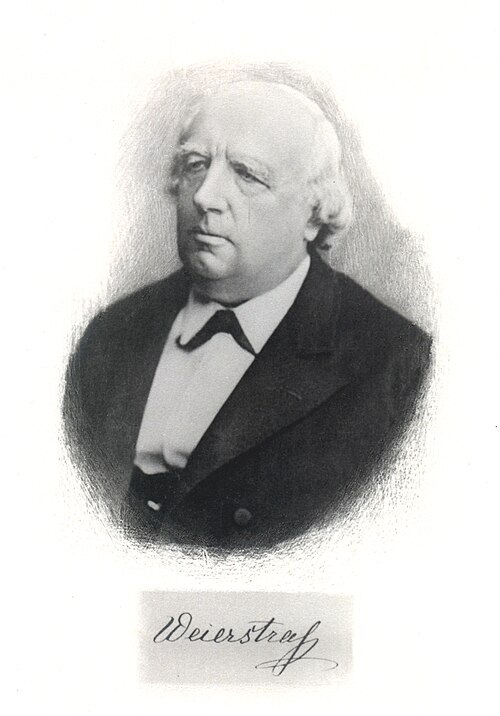
\includegraphics[width=0.88\textwidth]{weierstrass.jpg}
    \caption*{(a) \textbf{Karl Weierstrass (1815--1897)}}
  \end{minipage}
  \hfill
  \begin{minipage}{0.30\textwidth}
    \centering
    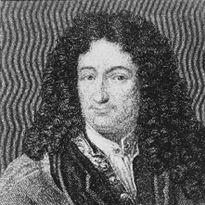
\includegraphics[width=0.88\textwidth]{rolle.jpg}
    \caption*{(b) \textbf{Michel Rolle (1652--1719)}}
  \end{minipage}
  \hfill
  \begin{minipage}{0.30\textwidth}
    \centering
    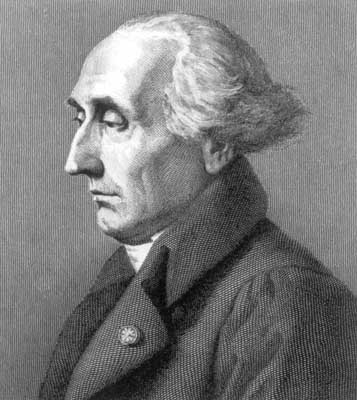
\includegraphics[width=0.88\textwidth]{lagrange.jpg}
    \caption*{(c) \textbf{Joseph-Louis Lagrange (1736--1813)}}
  \end{minipage}
  \caption{\textbf{Masters of Differential Calculus:} Karl Weierstrass ("Father of Modern Analysis", creator of the static $\varepsilon$-$\delta$ definition), Michel Rolle (formulator of Rolle's Theorem in 1691), and Joseph-Louis Lagrange (discoverer of the Mean Value Theorem and remainder formulas for Taylor series).}
  \label{fig:analysis_masters}
\end{figure}

\begin{definitionbox}{Formal $\varepsilon$-$\delta$ Definition of Functional Limit}
The function $f$ has a \textbf{limit} $L \in \mathbb{R}$ as $x$ approaches $x_0$, written $\lim_{x \to x_0} f(x) = L$, if:
\begin{equation}
\forall \varepsilon > 0, \quad \exists \delta > 0 \quad \text{such that} \quad \forall x \in I, \quad \left( 0 < |x - x_0| < \delta \implies |f(x) - L| < \varepsilon \right).
\end{equation}
\end{definitionbox}

\begin{figure}[htbp]
  \centering
  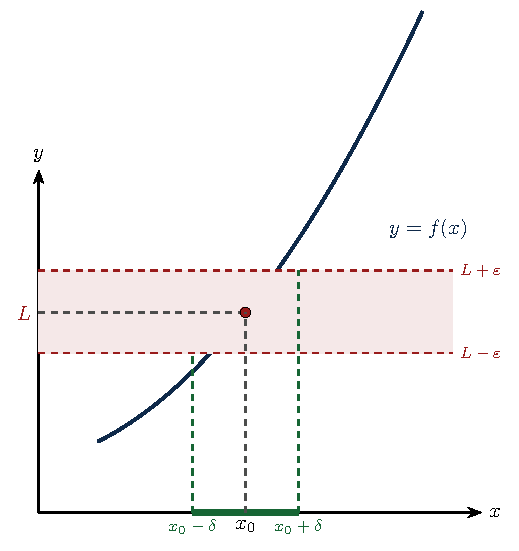
\includegraphics[width=0.88\textwidth]{05_epsilon_delta_limit.pdf}
  \caption{\textbf{Weierstrass $\varepsilon$-$\delta$ Neighborhood Geometry:} For any target band $(L - \varepsilon, L + \varepsilon)$ along the $y$-axis, there exists a surrounding interval $(x_0 - \delta, x_0 + \delta)$ on the $x$-axis whose functional images fall strictly within the band.}
  \label{fig:eps_delta}
\end{figure}

\begin{theorembox}{Sequential Characterization of Functional Limits (Heine's Theorem)}
Let $f: I \longrightarrow \mathbb{R}$ and $x_0$ an accumulation point of $I$. The following assertions are logically equivalent:
\begin{enumerate}[leftmargin=1.4em,itemsep=2pt]
  \item $\lim_{x \to x_0} f(x) = L$;
  \item For every sequence $(x_n)_{n \in \mathbb{N}}$ in $I \setminus \{x_0\}$ converging to $x_0$, the image sequence $(f(x_n))$ converges to $L$:
  \[
  \forall (x_n) \subset I \setminus \{x_0\}, \quad \left( \lim_{n \to \infty} x_n = x_0 \implies \lim_{n \to \infty} f(x_n) = L \right).
  \]
\end{enumerate}
\textit{Corollary (Disproof Criterion):} If two sequences $x_n \to x_0$ and $x'_n \to x_0$ yield different limits $\lim f(x_n) \neq \lim f(x'_n)$, then $\lim_{x \to x_0} f(x)$ does not exist (e.g. $f(x) = \sin(1/x)$ as $x \to 0$).
\end{theorembox}

\section{Continuity of Real Functions}

\begin{definitionbox}{Continuity at a Point and on an Interval}
\begin{enumerate}[leftmargin=1.4em,itemsep=3pt]
  \item A function $f: I \longrightarrow \mathbb{R}$ is \textbf{continuous at a point} $x_0 \in I$ if:
  \[
  \lim_{x \to x_0} f(x) = f(x_0) \iff \forall \varepsilon > 0, \ \exists \delta > 0, \ \forall x \in I, \ (|x - x_0| < \delta \implies |f(x) - f(x_0)| < \varepsilon).
  \]
  \item $f$ is \textbf{continuous on the interval} $I$ if it is continuous at every point $x_0 \in I$. We write $f \in \mathcal{C}^0(I)$ or $f \in \mathcal{C}(I, \mathbb{R})$.
\end{enumerate}
\end{definitionbox}

\begin{theorembox}{The Intermediate Value Theorem (Théorème des Valeurs Intermédiaires)}
Let $f: [a, b] \longrightarrow \mathbb{R}$ be a continuous function on a closed bounded interval $[a, b]$.
\begin{enumerate}[leftmargin=1.4em,itemsep=2pt]
  \item For every real number $y$ lying between $f(a)$ and $f(b)$, there exists at least one real number $c \in [a, b]$ such that:
  \[
  f(c) = y.
  \]
  \item \textbf{Bolzano's Root Theorem:} If $f(a) \cdot f(b) < 0$ (opposite signs at endpoints), then there exists at least one root $c \in (a, b)$ such that $f(c) = 0$.
\end{enumerate}
\end{theorembox}

\begin{theorembox}{The Extreme Value Theorem (Weierstrass's Theorem)}
Let $f: [a, b] \longrightarrow \mathbb{R}$ be a continuous function on a compact (closed and bounded) interval $[a, b]$.
Then $f$ is \textbf{bounded} and \textbf{attains its bounds}:
\begin{equation}
\exists x_{\min}, x_{\max} \in [a, b] \quad \text{such that} \quad f(x_{\min}) = \inf_{x \in [a, b]} f(x) \quad \text{and} \quad f(x_{\max}) = \sup_{x \in [a, b]} f(x).
\end{equation}
Thus, $f([a, b]) = [m, M]$ is itself a closed and bounded interval.
\end{theorembox}

\section{Differential Calculus: Definitions and Core Properties}

\begin{definitionbox}{The Derivative at a Point}
Let $f: I \longrightarrow \mathbb{R}$ and $x_0$ an interior point of $I$.
The function $f$ is \textbf{differentiable at $x_0$} if the difference quotient has a finite limit as $h \to 0$:
\begin{equation}
f'(x_0) = \lim_{h \to 0} \frac{f(x_0 + h) - f(x_0)}{h} = \lim_{x \to x_0} \frac{f(x) - f(x_0)}{x - x_0}.
\end{equation}
$f'(x_0)$ is the \textbf{derivative} of $f$ at $x_0$.
Geometrically, $f'(x_0)$ is the exact slope of the tangent line to the curve $y = f(x)$ at $(x_0, f(x_0))$:
\[
y = f(x_0) + f'(x_0)(x - x_0).
\]
\end{definitionbox}

\begin{theorembox}{Differentiability Implies Continuity}
If $f$ is differentiable at $x_0$, then $f$ is necessarily continuous at $x_0$:
\begin{equation}
f \text{ differentiable at } x_0 \implies f \text{ continuous at } x_0.
\end{equation}
(\textit{Caution:} The converse is false! The absolute value function $f(x) = |x|$ is continuous at $x = 0$ but not differentiable at $x = 0$).
\end{theorembox}

\begin{propbox}{Algebra of Derivatives}
Let $u, v: I \longrightarrow \mathbb{R}$ be differentiable at $x$:
\begin{enumerate}[leftmargin=1.4em,itemsep=2pt]
  \item \textbf{Linearity:} $(\alpha u + \beta v)'(x) = \alpha u'(x) + \beta v'(x)$ for all $\alpha, \beta \in \mathbb{R}$.
  \item \textbf{Leibniz Product Rule:} $(u \cdot v)'(x) = u'(x) v(x) + u(x) v'(x)$.
  \item \textbf{Quotient Rule:} $\left( \frac{u}{v} \right)'(x) = \frac{u'(x) v(x) - u(x) v'(x)}{[v(x)]^2}$ (provided $v(x) \neq 0$).
  \item \textbf{Chain Rule:} If $f$ is differentiable at $x$ and $g$ is differentiable at $f(x)$:
  \[
  (g \circ f)'(x) = g'(f(x)) \cdot f'(x).
  \]
  \item \textbf{Derivative of Inverse Function:} If $f$ is a bijective differentiable function with $f'(x_0) \neq 0$:
  \[
  (f^{-1})'(y_0) = \frac{1}{f'(x_0)} = \frac{1}{f'(f^{-1}(y_0))} \quad \text{where } y_0 = f(x_0).
  \]
\end{enumerate}
\end{propbox}

\section{Fundamental Theorems of Differential Calculus}

\begin{theorembox}{Fermat's Theorem on Local Extrema}
Let $f: (a, b) \longrightarrow \mathbb{R}$ be differentiable on the open interval $(a, b)$.
If $f$ attains a **local extremum** (local maximum or local minimum) at an interior point $c \in (a, b)$, then:
\begin{equation}
f'(c) = 0.
\end{equation}
Points where $f'(c) = 0$ are called \textbf{critical points} (or stationary points).
\end{theorembox}

\begin{figure}[htbp]
  \centering
  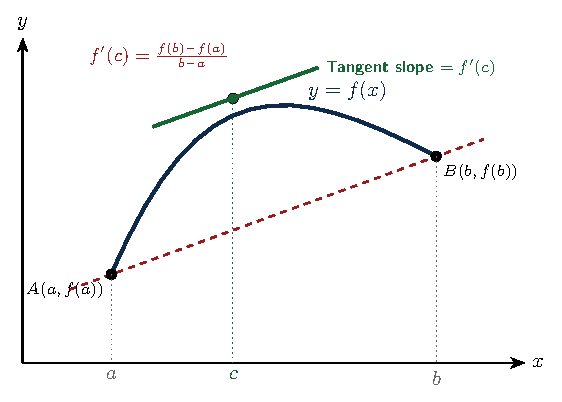
\includegraphics[width=0.88\textwidth]{06_rolle_mvt.pdf}
  \caption{\textbf{Rolle's and Mean Value Theorem Geometry:} The secant chord connecting endpoint coordinates $(a, f(a))$ and $(b, f(b))$ has slope $\frac{f(b) - f(a)}{b - a}$. There exists at least one interior point $c \in (a, b)$ where the tangent line to the curve is strictly parallel to the secant line ($f'(c) = \text{slope}$).}
  \label{fig:rolle_mvt}
\end{figure}

\begin{theorembox}{Rolle's Theorem (1691)}
Let $f: [a, b] \longrightarrow \mathbb{R}$ be a function satisfying:
\begin{enumerate}[leftmargin=1.4em,itemsep=2pt]
  \item $f$ is continuous on the closed interval $[a, b]$;
  \item $f$ is differentiable on the open interval $(a, b)$;
  \item $f(a) = f(b)$.
\end{enumerate}
Then there exists at least one interior point $c \in (a, b)$ such that:
\begin{equation}
f'(c) = 0.
\end{equation}
\end{theorembox}

\begin{theorembox}{The Mean Value Theorem (Théorème des Accroissements Finis / TAF)}
Let $f: [a, b] \longrightarrow \mathbb{R}$ be continuous on $[a, b]$ and differentiable on $(a, b)$.
Then there exists at least one point $c \in (a, b)$ such that:
\begin{equation}
f(b) - f(a) = f'(c) \cdot (b - a) \iff f'(c) = \frac{f(b) - f(a)}{b - a}.
\end{equation}
\end{theorembox}

\begin{propbox}{Corollaries of the Mean Value Theorem}
Let $f$ be differentiable on an interval $I$:
\begin{enumerate}[leftmargin=1.4em,itemsep=2pt]
  \item \textbf{Constant Function Criterion:} $\forall x \in I, f'(x) = 0 \iff f$ is constant on $I$.
  \item \textbf{Monotonicity Criteria:}
  \begin{itemize}[leftmargin=1.2em,itemsep=1pt]
    \item $f'(x) \ge 0$ on $I \iff f$ is monotonically increasing on $I$.
    \item $f'(x) \le 0$ on $I \iff f$ is monotonically decreasing on $I$.
    \item $f'(x) > 0$ on $I \implies f$ is strictly increasing on $I$.
  \end{itemize}
  \item \textbf{Mean Value Inequality (Inégalité des Accroissements Finis):}
  If $|f'(x)| \le M$ for all $x \in I$, then for all $x, y \in I$:
  \[
  |f(x) - f(y)| \le M |x - y|.
  \]
  (The function is Lipschitz continuous with Lipschitz constant $M$).
\end{enumerate}
\end{propbox}

\begin{theorembox}{Cauchy's Generalized Mean Value Theorem and L'Hôpital's Rule}
\begin{enumerate}[leftmargin=1.4em,itemsep=3pt]
  \item \textbf{Cauchy's Extended Mean Value Theorem:}
  If $f, g: [a, b] \longrightarrow \mathbb{R}$ are continuous on $[a, b]$ and differentiable on $(a, b)$, and $g'(x) \neq 0$ on $(a, b)$, then there exists $c \in (a, b)$ such that:
  \[
  \frac{f(b) - f(a)}{g(b) - g(a)} = \frac{f'(c)}{g'(c)}.
  \]
  \item \textbf{L'Hôpital's Rule:} If $\lim_{x \to x_0} f(x) = \lim_{x \to x_0} g(x) = 0$ (or $\pm\infty$), and $\lim_{x \to x_0} \frac{f'(x)}{g'(x)} = L \in \mathbb{R} \cup \{\pm\infty\}$, then:
  \[
  \lim_{x \to x_0} \frac{f(x)}{g(x)} = \lim_{x \to x_0} \frac{f'(x)}{g'(x)} = L.
  \]
\end{enumerate}
\end{theorembox}

\section{Worked Examples with Step-by-Step Proofs}

\begin{workedexample}{Rigorous Proof of Rolle's Theorem from Weierstrass's Theorem}
Provide the complete, rigorous analytical proof of Rolle's Theorem using the Extreme Value Theorem and Fermat's Theorem.

\paragraph{Solution and Proof.}
Let $f: [a, b] \longrightarrow \mathbb{R}$ satisfy the three hypotheses of Rolle's Theorem:
(1) $f$ is continuous on $[a, b]$, (2) $f$ is differentiable on $(a, b)$, and (3) $f(a) = f(b)$.

By the **Weierstrass Extreme Value Theorem**, because $f$ is continuous on the compact interval $[a, b]$, it is bounded and attains both its absolute minimum $m$ and absolute maximum $M$ at points $x_{\min}, x_{\max} \in [a, b]$:
\[
m = f(x_{\min}) = \min_{x \in [a, b]} f(x), \qquad M = f(x_{\max}) = \max_{x \in [a, b]} f(x).
\]
We now examine two mutually exclusive and exhaustive cases:
\begin{itemize}[leftmargin=1.4em,itemsep=3pt]
  \item \textbf{Case 1: $m = M$ (Constant Function).}
  If the minimum equals the maximum, then for all $x \in [a, b]$, $m \le f(x) \le M \implies f(x) = m$.
  Thus $f$ is a constant function on $[a, b]$.
  Its derivative is identically zero everywhere on $(a, b)$:
  \[
  \forall x \in (a, b), \quad f'(x) = 0.
  \]
  Any point $c \in (a, b)$ satisfies $f'(c) = 0$.

  \item \textbf{Case 2: $m < M$ (Non-constant Function).}
  Since $f(a) = f(b)$, it is impossible for both extrema to occur simultaneously at the boundary endpoints $\{a, b\}$.
  Indeed, if both occurred at the endpoints, we would have $m = f(a) = f(b) = M$, which contradicts $m < M$.
  Therefore, at least one of the two extrema must occur at an **interior point** $c \in (a, b)$:
  \begin{itemize}[leftmargin=1.2em,itemsep=1pt]
    \item Either $x_{\max} \in (a, b)$, in which case we set $c = x_{\max}$;
    \item Or $x_{\min} \in (a, b)$, in which case we set $c = x_{\min}$.
  \end{itemize}
  Since $c \in (a, b)$, $f$ has a local extremum at the interior point $c$.
  Moreover, by hypothesis (2), $f$ is differentiable at $c$.
  By **Fermat's Theorem on Local Extrema**, the derivative at an interior extremum must vanish:
  \[
  f'(c) = 0.
  \]
\end{itemize}
In both cases, we have established the existence of at least one point $c \in (a, b)$ such that $\mathbf{f'(c) = 0}$. $\blacksquare$
\end{workedexample}

\begin{workedexample}{Rigorous Proof of the Mean Value Theorem from Rolle's Theorem}
Derive the Mean Value Theorem by constructing an auxiliary function that satisfies Rolle's Theorem.

\paragraph{Solution and Proof.}
Let $f: [a, b] \longrightarrow \mathbb{R}$ be continuous on $[a, b]$ and differentiable on $(a, b)$.
The secant line connecting $(a, f(a))$ and $(b, f(b))$ has equation:
\[
y = f(a) + \frac{f(b) - f(a)}{b - a}(x - a).
\]
Consider the auxiliary function $\phi: [a, b] \longrightarrow \mathbb{R}$ measuring the vertical deviation between the curve $y = f(x)$ and the secant line:
\[
\phi(x) = f(x) - \left[ f(a) + \frac{f(b) - f(a)}{b - a}(x - a) \right].
\]
Let us verify the three hypotheses of Rolle's Theorem for $\phi$:
\begin{enumerate}[leftmargin=1.4em,itemsep=2pt]
  \item \textbf{Continuity on $[a, b]$:} $\phi$ is the difference of $f$ (continuous on $[a, b]$) and an affine linear function (continuous on $\mathbb{R}$). Hence $\phi$ is continuous on $[a, b]$.
  \item \textbf{Differentiability on $(a, b)$:} $\phi$ is differentiable on $(a, b)$ as the difference of differentiable functions, with derivative:
  \[
  \phi'(x) = f'(x) - \frac{f(b) - f(a)}{b - a}.
  \]
  \item \textbf{Equal Endpoint Values:}
  \[
  \phi(a) = f(a) - \left[ f(a) + \frac{f(b) - f(a)}{b - a}(a - a) \right] = f(a) - f(a) = 0.
  \]
  \[
  \phi(b) = f(b) - \left[ f(a) + \frac{f(b) - f(a)}{b - a}(b - a) \right] = f(b) - [f(a) + f(b) - f(a)] = 0.
  \]
  Thus $\phi(a) = \phi(b) = 0$.
\end{enumerate}
All three conditions of Rolle's Theorem are satisfied by $\phi$.
Therefore, there exists at least one point $c \in (a, b)$ such that:
\[
\phi'(c) = 0 \implies f'(c) - \frac{f(b) - f(a)}{b - a} = 0 \implies \mathbf{f'(c) = \frac{f(b) - f(a)}{b - a}}. \quad \blacksquare
\]
\end{workedexample}

\begin{workedexample}{Proving Classical Inequalities via the Mean Value Theorem}
Using the Mean Value Theorem:
\begin{enumerate}[leftmargin=1.4em,itemsep=2pt]
  \item Prove that for all real numbers $x > 0$:
  \[
  \frac{x}{1 + x} < \ln(1 + x) < x.
  \]
  \item Prove that for all $x \in \mathbb{R}$, $|\sin x| \le |x|$.
\end{enumerate}

\paragraph{Solution and Proof.}
\textbf{1. Logarithmic Inequality:}
Fix $x > 0$ and consider the function $f(t) = \ln(1 + t)$ on the interval $[0, x]$.
\begin{itemize}[leftmargin=1.4em,itemsep=2pt]
  \item $f$ is continuous on $[0, x]$ and differentiable on $(0, x)$, with derivative $f'(t) = \frac{1}{1 + t}$.
  \item By the Mean Value Theorem, there exists $c \in (0, x)$ such that:
  \[
  \frac{f(x) - f(0)}{x - 0} = f'(c) \implies \frac{\ln(1 + x) - \ln(1)}{x} = \frac{1}{1 + c} \implies \ln(1 + x) = \frac{x}{1 + c}.
  \]
  \item Since $0 < c < x$, we have $1 < 1 + c < 1 + x$.
  Inverting the inequalities:
  \[
  \frac{1}{1 + x} < \frac{1}{1 + c} < 1.
  \]
  Multiplying through by $x > 0$:
  \[
  \mathbf{\frac{x}{1 + x} < \ln(1 + x) < x}.
  \]
\end{itemize}

\textbf{2. Sine Inequality:}
Consider $g(t) = \sin t$.
For $x = 0$, $|\sin 0| = 0 \le 0$ holds trivially.
For $x \neq 0$, apply the Mean Value Theorem on the interval between $0$ and $x$:
\[
\frac{\sin x - \sin 0}{x - 0} = \cos(c) \quad \text{for some } c \text{ between } 0 \text{ and } x.
\]
Taking absolute values:
\[
\frac{|\sin x|}{|x|} = |\cos c|.
\]
Since $|\cos c| \le 1$ for all real $c$:
\[
\frac{|\sin x|}{|x|} \le 1 \implies \mathbf{|\sin x| \le |x|}. \quad \blacksquare
\]
\end{workedexample}

\begin{workedexample}{Bijective Inverse Function Derivative}
Consider the function $f: \mathbb{R} \longrightarrow \mathbb{R}$ defined by:
\[
f(x) = x^3 + 2x - 1.
\]
\begin{enumerate}[leftmargin=1.4em,itemsep=2pt]
  \item Prove that $f$ is a bijection from $\mathbb{R}$ onto $\mathbb{R}$.
  \item Calculate $f(1)$.
  \item Compute the derivative of the inverse function at $y_0 = 2$, namely $(f^{-1})'(2)$.
\end{enumerate}

\paragraph{Solution and Proof.}
\textbf{1. Proof of Bijectivity:}
$f$ is a polynomial, hence continuous and infinitely differentiable on $\mathbb{R}$.
Its derivative is:
\[
f'(x) = 3x^2 + 2.
\]
For all $x \in \mathbb{R}$, $3x^2 \ge 0 \implies f'(x) \ge 2 > 0$.
Since $f'(x) > 0$ everywhere, $f$ is **strictly increasing** on $\mathbb{R}$.
Furthermore, examining limits at infinity:
\[
\lim_{x \to -\infty} f(x) = -\infty, \qquad \lim_{x \to +\infty} f(x) = +\infty.
\]
By the **Continuous Bijection Theorem**, a strictly increasing continuous function on $\mathbb{R}$ is a bijection from $\mathbb{R}$ onto $\mathbb{R}$.

\textbf{2. Evaluation at $x = 1$:}
\[
f(1) = 1^3 + 2(1) - 1 = 1 + 2 - 1 = \mathbf{2}.
\]

\textbf{3. Derivative of the Inverse Function at $y_0 = 2$:}
Since $f(1) = 2$, we have $f^{-1}(2) = 1$.
Using the formula for the derivative of the inverse function:
\[
(f^{-1})'(2) = \frac{1}{f'(f^{-1}(2))} = \frac{1}{f'(1)}.
\]
Compute $f'(1)$:
\[
f'(1) = 3(1)^2 + 2 = 3 + 2 = 5 \neq 0.
\]
Therefore:
\[
\mathbf{(f^{-1})'(2) = \frac{1}{5} = 0.2}. \quad \blacksquare
\]
\end{workedexample}
